%----------------------------------------------------------------------------
\chapter{Managing Cosmos DB with Azure Functions}\label{Ch4}
%----------------------------------------------------------------------------

The backend of my application consists of five microservices. I will explain the creation of a microservice, then I will get on to my exact solution.  
%----------------------------------------------------------------------------
\section{Creating a Microservice with Azure Functions}
%----------------------------------------------------------------------------
In this case by microservice we will mean an Azure Function App. 
These are the steps for creating a new Azure Functions microservice: \cite{VSCodeFunction}

\begin{enumerate}
	\item Open an empty folder in VS Code.
	\item Hit F1 and choose Azure Functions: Create new project...
	\item Choose \verb+C#+ with .NET 6.0 LTS.
	\item To create the first Azure Function in the project, choose a trigger type. In this example I chose HTTP Trigger.
	\item Give it a name and select a namespace. My function is called AddReview and the namespace will be Review. Set Anonymous access rights.
\end{enumerate}
	
Now we have an Azure project with a basic Azure Function generated. It can be tested by hitting F5 in the console. All of our functions will be listed with their routes included, but for now we only have one: http://localhost:7071/api/AddReview. When we call it, we get the following response: (See Figure \figref{res})

\begin{figure}[!ht]
	\centering
	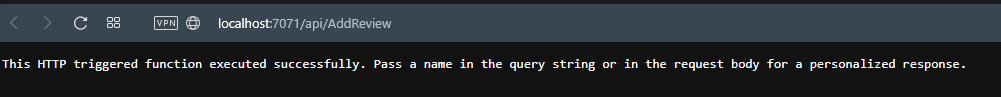
\includegraphics[width=150mm, keepaspectratio]{figures/4_response.png}
	\caption{Calling the function successfully.} 
	\label{fig:res}
\end{figure}

At this point we are free to make modifications to this function and then upload it to the cloud. But before publishing, we should create a Function App in Azure as this going to contain our functions. This can be achieved in VS Code as well. Hit F1 and choose \verb+Create Function App in Azure+ in the prompt. Sign in to Azure if needed and follow the instructions. I chose \verb+review-func-app+ as name, .NET 6 (non-isolated) runtime stack and a European location. When the resource is created, open again the Command Palette and choose \verb+Azure Functions: Deploy to Function App+ and select your freshly created function app. Click deploy and wait for the process to be finished, as this can take several minutes. At the bottom of the console output tab you should see the url to your published functions. They follow the pattern
\emph{https://your-func-app-name.azurewebsites.net/api/funcname}.

However calling these functions would end up giving an internal server error. Some modifications have to be made in the Azure Portal as well. These will be the following:
\begin{itemize}
	\item \textbf{Updating CORS}
	 In the search bar find your function app and on the sidebar, under API look for CORS. Here we type in all origins we would like to access this function app from, so the api will accept requests from these origins. I will add localhost with the default Angular port \emph{http://localhost:4200} and also the url of my published static app: \emph{https://ambitious-desert-085d2d503.1.azurestaticapps.net}. Save the modifications.
	 
	\item \textbf{Adding local settings to the portal}\label{LocalSettings}
	If the functions use (or will be using) Cosmos DB, then the connection string should be provided here and locally as well in \verb+local.settings.json+. Head to Configuration under Settings on the sidebar. Assuming that we already created a database, the connection string can be retrieved from multiple sources. In VS Code under Resources find your database, right click on it and choose Copy Connection String. In Azure Portal navigate to the Cosmos DB Account and on the sidebar under Settings select Keys and copy the Primary Connection String. Navigate back to the function app and add a New application setting, paste the Cosmos DB connection string under the value attribute and give it a name. Make sure to use this same name in your local settings and in your functions. Hit OK and Save the modifications.
\end{itemize}
  When all of this is finished, the function should work properly, in my case I could add a new review. (See Figure \figref{res_pub})

\begin{figure}[!ht]
	\centering
	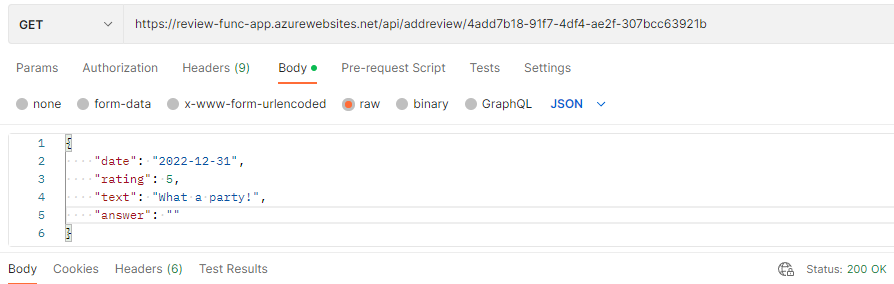
\includegraphics[width=150mm, keepaspectratio]{figures/7_published_response.png}
	\caption{Calling the function after publication.}
	\label{fig:res_pub}
\end{figure}

I did a small additional step, which is optional. I set up continuous deployment with GitHub Actions \cite{GitHubActionsForFunctions}, so every time I push the project to GitHub, it will be deployed automatically. This goes really quickly:

\begin{enumerate}
	\item Create an empty GitHub repository.
	\item Push the function app (its folder is initialized by default).
	\item Log in to Azure Portal at \url{https://portal.azure.com} and find the created function app.
	\item Navigate to Deployment Center on the sidebar.
	\item Select GitHub as source and authenticate with it.
	\item Select the function app's repository and a branch, whose content will be deployed.
	\item When you hit save, Azure will add a .yml file to the repository.
	\item Don't forget to pull this locally to avoid merge conflict.
	\item Modify the project and push it to GitHub.
\end{enumerate}

The changes should be deployed within a few minutes. (This process can be followed at the GitHub repository's Actions tab.)

%----------------------------------------------------------------------------
\section{Setting up a connection with Cosmos DB}
%----------------------------------------------------------------------------

Cosmos DB \cite{CosmosDBIntro} is a fully managed NoSQL database and compatible with multiple database APIs as Mongo DB, the native NoSQL API but also has relational database options. Fully managed in a sense that the user only has to create a resource in Azure and the database is ready to use, no further maintenance is needed (as previously mentioned in the Introduction). It is advertised with 99.999\% availability time and enterprise-grade security. Cosmos DB supports querying NoSQL API databases with SQL, in case of .NET Linq is also supported. 

Nearly all services will rely on some kind of data storage. In this case the application data is stored in Cosmos DB. The new database creation steps differ slightly based on the used framework and database API, but it has a solid documentation discussing all the options \cite{CosmosDBQuickstart}. If we would like to reach the created database from Azure Functions, we need an additional extension \ref{addCosmosDB} (see more detail at \cite{CosmosDBBinding}).

\lstset{ breaklines=true }
\begin{lstlisting}[frame=single,float=!ht, caption=Adding Cosmos DB to a Function App, label=addCosmosDB]
	dotnet add package Microsoft.Azure.WebJobs.Extensions.CosmosDB
\end{lstlisting}

My database structure is the following: the database file is called \emph{Restaurant} and includes three collections, \emph{RestaurantItems}, \emph{Orders} and \emph{Users}. These contain the single restaurant, order or user \emph{items} (read more about the Cosmos DB resource model here: \cite{CosmosDBResourceModel}). If we install the Azure Databases VS Code extension, we will be able to make changes and follow the database's state from the code editor's Azure tab by opening up the Resources dropdown (see image \figref{CosmosStructure}). 
\begin{figure}[!ht]
	\centering
	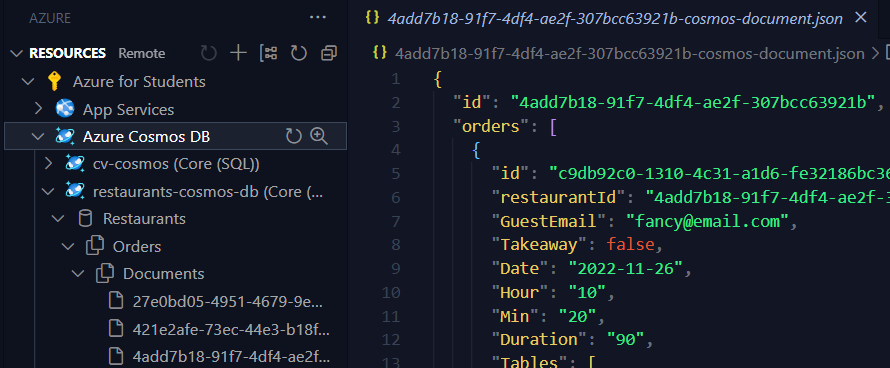
\includegraphics[width=150mm, keepaspectratio]{figures/DB/CosmosStructure.png}
	\caption{The database structure from VS Code} 
	\label{fig:CosmosStructure}
\end{figure}


%----------------------------------------------------------------------------
\section{Microservices}
%----------------------------------------------------------------------------
Now we proceed to discuss the app's services.
%----------------------------------------------------------------------------
\subsection{Auth Microservice}\label{RestaurantMicroservice}
%----------------------------------------------------------------------------

Auth Microservice is published at \ref{AuthMs}. It manages the user accounts, which are stored in the database's Users collection:

\begin{enumerate}
	\item \verb+AddUser+: Creates a new user document in the collection from the received JSON. 
	
	\item \verb+GetUserByEmail+: It performs a point read by the e-mail it gets in the route and returns the found user if any. E-mails are used as ids in this collection.
	
\end{enumerate}
Additional files:
\begin{enumerate}
	\item \verb+User.cs+: Describes the data structure of a user account.
\end{enumerate}

%----------------------------------------------------------------------------
\subsection{Restaurant Microservice}\label{RestaurantMicroservice}
%----------------------------------------------------------------------------
Restaurant Microservice is published at \ref{RestaurantMs}. It handles the RestaurantItems database collection and contains the following functions:

\begin{enumerate}
	\item \verb+GetAllRestaurants+: The function binds to the RestaurantItem collection and queries all of its items. Read more about Cosmos DB input binding here: \cite{CosmosDBInputBinding}
	\item \verb+GetRestaurantsWithFilter+: Works the same way as GetAllRestaurants, but parameters e.g.\ maxprice, rating can be sent to it. The function converts these to the wished format and filters the query results according to the given criteria.
	
	\item \verb+RestaurantById+: 
	It performs a point read by the id data it gets in the route and returns the result. Point reads are more cost effective than querying, so it is a good rule of thumb to use them whenever applicable \cite{CosmosDBCostOpt}. In my case the id and the partitionKey has the same value, but this is only because on creation I set up the container so. Overall, it is a good idea to set the id as partition key value, but note that it's not true to every database (find more on partitioning here: \cite{CosmosDBPartitioning}). 
	
	\item \verb+AddRestaurantOrchestration+: 
	This is a durable function orchestrator. Durable functions allow the developer to make chained or parallel function calls. I used the function chaining pattern here, which means that when the orchestrator is called, it will call the first function, waits to the evaluation then passes the result to the next function in the row (read more about the concept of durable functions here: \cite{DurableFunctions}).
	
	A durable function's entry point is a HttpStart function (by default gets the name myfunction\_HttpStart). It will call the orchestrator, wait for its execution and return the result. If we would like to pass JSON data to the functions called by the orchestrator, we should send it to the starter function, read the request data and pass it on as it is. The orchestrator can call functions in the same function app by their name or from anywhere else by their url. Read more about implementation details here: \cite{DurableFunctionsImplement}.
	
	How does this work in the context of our application? The function gets called, when a new restaurant is created by a user. It accomplishes three things: calls the \emph{AddRestaurantActivity}, which creates a new restaurant item document from the data that was sent in the request body. Generates a new id for it and adds it to the \emph{RestaurantItems} collection. This new id is returned back to the orchestrator and with it the \emph{addOrderRestaurant} function from the Order function app can be called, which creates an empty orders list for the restaurant. Finally, Auth function app's \emph{AddUser} function creates a new user with the restaurant's basic infos and generated id (see Figure \figref{durable}).	
	
	\begin{figure}[!ht]
		\centering
		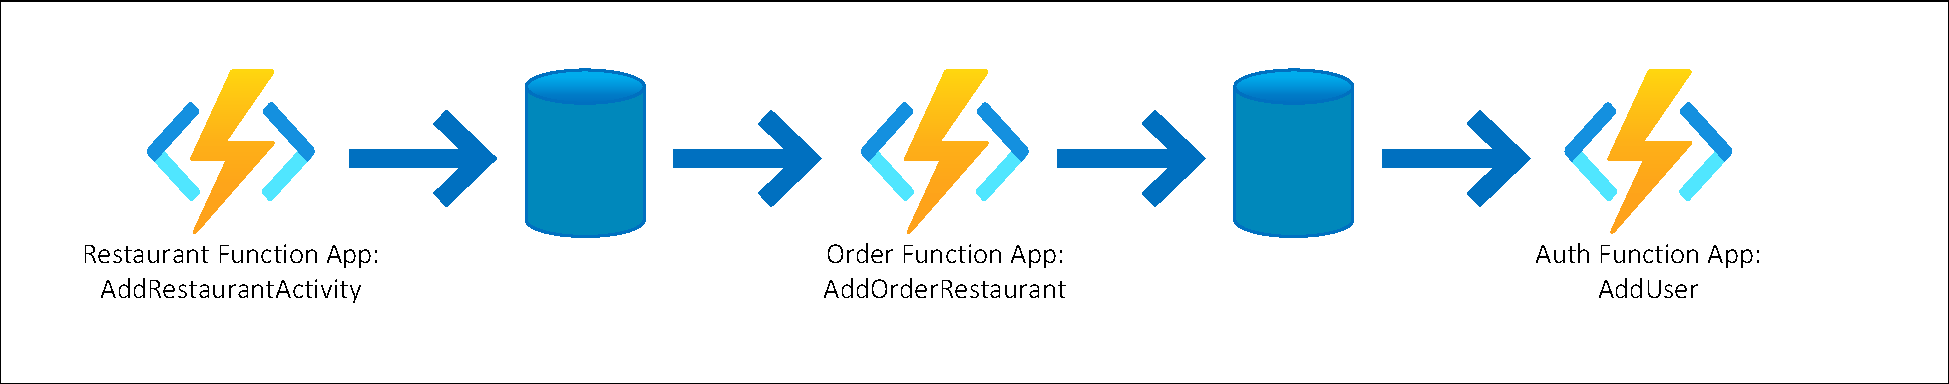
\includegraphics[width=150mm, keepaspectratio]{figures/Durable}
		\caption{Calls made by the orchestrator function} 
		\label{fig:durable}
	\end{figure}
	
\end{enumerate}

Additional files: 

\begin{enumerate}
	\item \verb+Restaurant.cs+: Contains the RestaurantItem class and some nested classes as Review or MenuItem. These describe the structure of the restaurantItem documents in Cosmos DB that's why the class contains the id and partitionKey attributes.
\end{enumerate}

%----------------------------------------------------------------------------
\subsection{Review Microservice}\label{ReviewMicroservice}
%----------------------------------------------------------------------------

Review Microservice is published at \ref{ReviewMs}. It handles the RestaurantItems collection's Reviews list. I decided to handle it separately as reviews are added to the document independently and seemed to form an independent unit logically. Although I didn't separate the database document, which at the time saved some coding but later turned out to be inconvenient. It would be better with a setup like in Order microservice even more so, because the Reviews list can grow boundlessly which can lead to problems \cite{NoSQLArrays}. The function app contains the following functions:

\begin{enumerate}
	\item \verb+AddReview+: This function saves user reviews of a restaurant. I used here the relatively new Partial Document Update feature, which allows us to modify an existing Cosmos DB document in one operation (see \cite{CosmosDBPartialDocumentUpdate}). This can be accessed via \ref{partialDoc}. 
	
	\lstset{ breaklines=true }
	\begin{lstlisting}[frame=single,float=!ht, caption=Adding Partial Document Update to a Function App, label=partialDoc]
		dotnet add package Microsoft.Azure.Cosmos
	\end{lstlisting}

	The AddReview function looks up the restaurantItem, whose id equals the id in the route. Then reads the review sent in the request body and creates a new review document, which will get the id with the current length of the restaurant's reviews list and then adds it to that exact index in the list. This solution is not flawless but I use it because partial document update can't manage array items by id, only by index. 	
	
	\emph{"If the target path is a valid array index, a new element will be inserted into the array at the specified index. It shifts existing elements to the right.
	If the index specified is equal to the length of the array, it will append an element to the array."  \cite{CosmosDBPartialDocumentUpdate}}
 	
	So if we would like to save ourselves from reading the list, finding the right item and get its index every time we have to update an item, then we should somehow store the index of each item. 
	
	This function class contains a few private attributes, I explain those later at the Startup.cs file's description.
	
	\item \verb+CalcRating+: Every time a new review is added by AddReview, it calls this function, which recalculates the connected restaurant's rating including the new review's rating. For this it reads the restaurant's reviews, sums up all reviews' rating and divides it by the review count, then updates the restaurant's rating attribute. Read more on output binding here: \cite{CosmosDBOutputBinding}
	I didn't use durable functions because it isn't a crucial task, if it runs successfully once in a while it will be enough.
	
	\item \verb+UpdateReview+: This function updates an already existing review. It is called, when a restaurant replies to a review. The function expects a review object in the request body and replaces it by its index (which we previously stored as the review's id). 
\end{enumerate}

Additional files: 

\begin{enumerate}
	\item \verb+Review.cs+: Contains the Review class and a RestaurantItem class, because the functions have to find the right restaurant item to read its reviews. This class only includes the attributes the review functions have to know about.
	
	\item \verb+Startup.cs+: Partial document update functions are accessible via the CosmosClient class, but unfortunately there is no support to bind it to an Azure Function. So we have to set it up in a separate Startup function, so the functions can retrieve them from here. Detailed steps about this can be found here: \cite{CosmosClient}
\end{enumerate}

%----------------------------------------------------------------------------
\subsection{Order Microservice}\label{OrderMicroservice}
%----------------------------------------------------------------------------

Order Microservice is published at \ref{OrderMs} and it handles the Orders collection. The collection's documents consist of a restaurant's id and a list of orders. 
I implemented the following functions:

\begin{enumerate}
	\item \verb+GetRestaurantOrders+: Reads and returns all orders from the document who's restaurant id equals the id in the route data. 
	
	\item \verb+GetOrdersToday+: Works the same way as GetRestaurantOrders, but filters the query results and returns only those, whose date equals the date route parameter's value.
	
	\item \verb+AddOrderRestaurant+: As I mentioned earlier, this function gets called by AddRestaurantOrchestration function, when a new restaurant was created. Gets the restaurant id as a route parameter and creates a new document with it. 
	
	\item \verb+AppendNewOrder+: It is called, when a user places a new order. The function creates an order object from the data it got in the request body. Then updates the orders list of the document whose id equals the order's restaurant id (with the help of partial document update).  

\end{enumerate}

Additional files: 

\begin{enumerate}
	\item \verb+Order.cs+: Containts the Order and OrderRestaurant classes. The latter consist of an id and an order list, the former gives the structure of an order.
	
	\item \verb+Startup.cs+: Same as in Review Microservice.
\end{enumerate}

%----------------------------------------------------------------------------
\subsection{Email Microservice}\label{EmailMicroservice}
%----------------------------------------------------------------------------

Email Microservice is published at \ref{EmailMs}. It sends out e-mails through the new Azure Communication Services. For this, I had to create a Communication Service resource \cite{CommunicationResource} and had to connect a domain to the resource \cite{ConnectEmailDomain}. I used an Azure domain, but a custom one can be set up as well. After installing the Azure Communication Services Email client library for .NET package (with the command \ref{addEmail}), we are ready to send e-mails \cite{SendEmail}. Note that this will only work locally. After publishing the function app, the connection string should be set in the Azure Portal too (the same way as the Cosmos DB connection string, we discussed it earlier here: \ref{LocalSettings}). 

\lstset{ breaklines=true }
\begin{lstlisting}[frame=single,float=!ht, caption=Adding the e-mail package to a Function App, label=addEmail]
	dotnet add package Azure.Communication.Email --prerelease 
\end{lstlisting}

 I created the following HTTP trigger functions:

\begin{enumerate}
	\item \verb+SendInvoiceEmail+: The function expects the e-mail data in the request body in the form of the \emph{EmailInvoice} class. Connects to the email client via the connection string, constructs the HTML content and sends the e-mail to the given e-mail address.
	
	\item \verb+SendOrderDetailsEmail+: Operates similarly to the previous function, but uses the EmailOrder class and the e-mail content differs.
	
	\item \verb+SendRegConfirmationEmail+: Used for confirming the e-mail address of a new guest. Sends the received code to the e-mail address.
\end{enumerate}

Additional files: 

\begin{enumerate}
	\item \verb+EmailData.cs+ file contains three classes, \emph{EmailOrder}, \emph{EmailInvoice} and \emph{EmailRegConfirmation}. They represent the collections of data sent in the corresponding e-mail type.
\end{enumerate}